%!TEX root = ../template.tex
%%%%%%%%%%%%%%%%%%%%%%%%%%%%%%%%%%%%%%%%%%%%%%%%%%%%%%%%%%%%%%%%%%%%
%% chapter3.tex
%% NOVA thesis document file
%%
%% Chapter with the template manual
%%%%%%%%%%%%%%%%%%%%%%%%%%%%%%%%%%%%%%%%%%%%%%%%%%%%%%%%%%%%%%%%%%%%

\typeout{NT FILE chapter3.tex}%

\chapter{Related work}\label{cha:related_work}

In this chapter we talk about work that has been developed and we found that is most in line with our work. We used them
either as a comparison to what we want to develop or as a part of the solution that
we are proposing.

In this Section we discuss some simulators that evaluated to be relevant to study
since they provide tools that are in line to what we also want to provide with MOBS and
are the state of the art for blockchain simulators.

\section{VIBES}~\label{subsec:vibes}

Vibes~\cite{vibes} is a message driven blockchain simulator developed with the goal of providing
configurable, scalable and fast network simulations. It also provides a GUI for visualization
of some extracted metrics and allows users to view a time-lapse of the processed events.

Vibes is developed in Scala and as such inherits the Actor language paradigm, the actors in
Vibes can have one of three roles:

\begin{itemize}
  \item \textbf{Node:} Follows the protocol to replicate the behavior of the blockchain
  network.
  \item \textbf{Coordinator:} This actor acts as an application-level schedule. It receives
  requests from all nodes to fast-forward the network to the point in time when each node
  has completed his current task and once it receives a request from all nodes it moves the
  entire network to the earliest timestamp, guaranteeing a correct execution order of all tasks.
  \item \textbf{Reducer:} Once the simulation ends the reducer gathers the state of the network
  and produces the simulation results to be processed by the user.
\end{itemize}

\section{BlockSim: Blockchain Simulator}~\label{subsec:blocksim1}

BlockSim~\cite{blocksim1} is a simulation framework that assists in the design and Evaluation
of blockchain protocols. Developed in Python it uses a probabilistic distributions model that
can be specified by the user to model random phenomena such as time taken to validate a block and
network latency.

\begin{figure}[h]
	\centering
	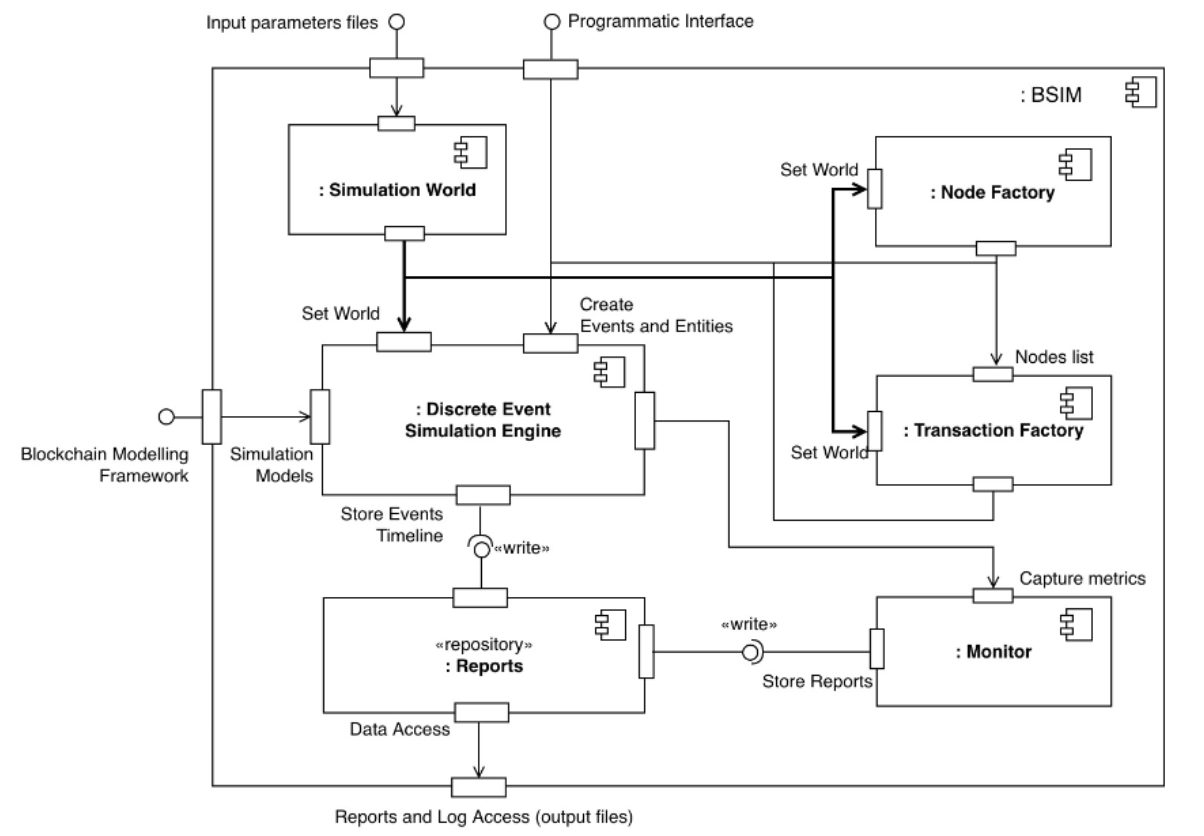
\includegraphics[width=4.5in, angle =0]{blocksim_fig}
	\caption{BlockSim Architecture~\cite{blocksim1}}
	\label{fig:blocksim_fig}
\end{figure}

BlockSim's architecture, as shown in the figure, is made up by the following components:

\begin{itemize}
  \item \textbf{DESE:} Discrete Event Simulation Engine, based on SimPy
  \item \textbf{Simulation World:} Responsible for handling input/configuration parameters
  of the simulations.
  \item \textbf{Transaction and Node Factory:} Responsible for creating batches of 
  transactions modelled as random phenomena. Node Factory creates nodes that are used 
  during the simulation
  \item \textbf{Programmatic interface and Simulation Example:} Main interface available to 
  the user
  \item \textbf{Monitor and reports:} Monitor captures metrics during the simulation, 
  i.e.\ number of transactions broadcasted or received, transactions added to queue. 
  These metrics are stored in the reports component
  \item \textbf{Blockchain modelling Framework:} Has several layers like the Node layer,
  the Consensus, the Ledger, Transaction and block, Network and Cryptographic.
\end{itemize}

\section{BlockSim: Extensible simulation tool for blockchain systems}~\label{subsec:blocksim2}

Although with a similar name of the previously presented simulator, BlockSim is a different 
framework designed to build and simulate discrete-event dynamic systems models for blockchain systems.

BlockSim has three main modules:
\begin{itemize}
  \item \textbf{Simulation:} Is in charge of setting up the scheduling of events and compute
  the simulation statistics.
  \item \textbf{Base:} Consists of the layers for the implementation of the blockchain protocol
  that will be simulated
  \item \textbf{Configuration:}  Is the main user interface where the simulation can be 
  selected and parameterized.
\end{itemize}

The base module has three layers that can be extended by the user:

\begin{itemize}
  \item \textbf{Network:} represents blockchain nodes and the underlying peer-to-peer protocol
  to exchange data.
  \item \textbf{Consensus:} encompasses algorithms and rules adopted to reach an agreement 
  about the current state of the blockchain ledger.
  \item \textbf{Incentives:} contains the economic incentive mechanisms adopted by a 
  blockchain to issue and distribute rewards among participating nodes.
\end{itemize}

\section{SimBlock:A Blockchain Network Simulator}~\label{subsec:simblock}

SimBlock was developed in Java to preform experiments on blockchain protocols
with a large amount of nodes. It allows users to easily change the behavior of nodes
and study their overall impact on the network. It also provides users with a simple GUI for
users to load the output file of a simulation and observe evolution of the simulated protocol.
Simblock is divided into three components:

\begin{itemize}
  \item \textbf{Network:} Creates the network topology which is configurable in the number
  of nodes, number of neighbors for each node and latency for each node to its neighbors.
  \item \textbf{Node:} Defines the behavior of each node in accordance to the simulated protocol.
  \item \textbf{Node:} Defines the rules for creating and validating blocks.
\end{itemize}

\section{JABS}~\label{subsec:jabs}

JABS~\cite{jabs} was developed in JAVA and is aimed at researching large-scale blockchain consensus algorithms, with a main focus
on simulating consensus, network, and ledger-data layers. The simulator is designed to be
modular and extensible, optimized for performance and scalability.

JABS is developed to be used as a discrete-event simulation tool for benchmarking, evaluating, adjusting,
and comparing consensus algorithms, especially for global-size public blockchains

JABS is composed of five main components:

\begin{itemize}
  \item \textbf{Scenario:} Serves as a template for designing and adjusting simulation parameters.
  \item \textbf{Network:} Describes the connections between nodes and their bandwidth.
  \item \textbf{Simulator:} Responsible for processing each node's events in the correct order.
  \item \textbf{Node:} Is where the logic for the protocol is implemented and defines each node's
  behavior
  \item \textbf{Logger:} Handles all the outputs in the simulation into either a standard output or
  a CSV file.
\end{itemize}


\section{Critical Analysis}~\label{subsec:critical_analysis}

We analyzed the presented simulators, either by reading the papers presented by the creators,
using the publicly available ones to run their implemented protocols or in the case of JABS, trying to
implement a new protocol to see how the creators provided modularity and extensibility. From that
analysis we compiled this data:

\begin{table}[h]
  \tiny
  \centering
  \begin{tabular}{|c|c|c|c|c|c|c|c|}
    \hline
    & \textbf{\begin{tabular}[c]{@{}c@{}}Adversarial\\ Behavior\end{tabular}} & \textbf{\begin{tabular}[c]{@{}c@{}}Offline \\ Nodes\end{tabular}} & \textbf{\begin{tabular}[c]{@{}c@{}}Bandwidth\\  Limits\end{tabular}}                      & \textbf{\begin{tabular}[c]{@{}c@{}}Network \\ Topology\end{tabular}}   & \textbf{Proof of Stake}                                   & \textbf{Proof of Work}                                                   & \textbf{GUI} \\ \hline
    \textbf{VIBES} \cite{vibes}   & yes                                                                     & \begin{tabular}[c]{@{}c@{}}not \\ modeled\end{tabular}            & \begin{tabular}[c]{@{}c@{}}not\\ modeled\end{tabular}                                     & \begin{tabular}[c]{@{}c@{}}generated \\ via \\ parameters\end{tabular} & \begin{tabular}[c]{@{}c@{}}not \\ modeled\end{tabular}    & bitcoin                                                                  & yes          \\ \hline
    \textbf{BlockSim} \cite{blocksim1} & \begin{tabular}[c]{@{}c@{}}not\\ modeled\end{tabular}                   & \begin{tabular}[c]{@{}c@{}}not \\ modeled\end{tabular}            & \begin{tabular}[c]{@{}c@{}}Throughput \\ calculated \\ from \\ distribution\end{tabular} & \begin{tabular}[c]{@{}c@{}}fully \\ linked\end{tabular}                & \begin{tabular}[c]{@{}c@{}}not \\ modeled\end{tabular}    & \begin{tabular}[c]{@{}c@{}}bitcoin \\ ethereum\end{tabular}              & no           \\ \hline
    \textbf{BlockSim} \cite{blocksim2} & \begin{tabular}[c]{@{}c@{}}not\\ modeled\end{tabular}                   & \begin{tabular}[c]{@{}c@{}}not \\ modeled\end{tabular}            & \begin{tabular}[c]{@{}c@{}}not \\ modeled\end{tabular}                                    & \begin{tabular}[c]{@{}c@{}}fully \\ linked\end{tabular}                & \begin{tabular}[c]{@{}c@{}}not \\ modeled\end{tabular}    & \begin{tabular}[c]{@{}c@{}}bitcoin \\ ethereum\end{tabular}              & no           \\ \hline
    \textbf{SimBlock} \cite{simblock} & \begin{tabular}[c]{@{}c@{}}not \\ modeled\end{tabular}                  & \begin{tabular}[c]{@{}c@{}}not \\ modeled\end{tabular}            & \begin{tabular}[c]{@{}c@{}}specify \\ expected \\ available \\ bandwidth\end{tabular}     & \begin{tabular}[c]{@{}c@{}}generated \\ via \\ params\end{tabular}     & \begin{tabular}[c]{@{}c@{}}simple \\ example\end{tabular} & \begin{tabular}[c]{@{}c@{}}bitcoin \\ dogecoin \\ litecoin\end{tabular}  & yes          \\ \hline
    \textbf{JABS} \cite{jabs} & \begin{tabular}[c]{@{}c@{}}not \\ modeled\end{tabular}                  & \begin{tabular}[c]{@{}c@{}}not \\ modeled\end{tabular}            & \begin{tabular}[c]{@{}c@{}}configurable\end{tabular}     & \begin{tabular}[c]{@{}c@{}}generated \\ via \\ network \\ layer\end{tabular}     & \begin{tabular}[c]{@{}c@{}}simple \\ example\end{tabular} & \begin{tabular}[c]{@{}c@{}}bitcoin \\ DAGsper\end{tabular}  & no          \\ \hline
    \textbf{MOBS}     & yes                                                                     & yes                                                               & parametrizable                                                                           & \begin{tabular}[c]{@{}c@{}}generated \\ via \\ params\end{tabular}     & tenderbake                                                & \begin{tabular}[c]{@{}c@{}}bitcoin \\ algorand \\ ouroboros\end{tabular} & yes          \\ \hline
    \end{tabular}
  \caption{Feature comparison between existing blockchain simulators and MOBS.}
\label{table:1}
\end{table}

In Vibes~\cite{vibes} there is a lack of separation between the code that defines the
simulator and the codes that defines the protocols, which makes implementing new
protocols difficult and time costly. On the GUI provided this lack of separation
also exists, having the statistics that are displayed tied to the protocols being
simulated, which means that if the user wants to implement a new protocol that has
different metrics/statistics, changes would need to be done to the GUI to support
them.

Neither BlockSim~\cite{blocksim1}, BlockSim~\cite{blocksim2}, SimBlock~\cite{simblock} nor
JABS support adversarial or Byzantine behavior
of the nodes, making it impossible to test the protocols when the network is not in
perfect conditions.

VIBEs, BlockSim and BlockSim do not model Proof of Stake protocols which hinders
their extensibility, since as a result, these simulators don't offer abstractions
for timers and alarms commonly used in proof of stake.

JABS designed to implement simple blockchain protocols, and is not ready to implement
pure consensus protocols. Furthermore, it lacks the means to leverage the already implemented
logic in other protocols to be re-used in new implementations, making the development of new
protocols costly and time-consuming.